% Fig.5: datapath measurement topology — a traffic generator drives
% line-rate traffic over 100 GbE into the DUT, whose native XDP program
% evaluates the filter and drops every packet. Filter cost is the
% processing-rate difference against an accept-all program on the same
% traffic.
% Build: pdflatex fig_topology.tex -> fig_topology.pdf
\documentclass[tikz]{standalone}
\usetikzlibrary{positioning, arrows.meta, fit, calc}
\begin{document}
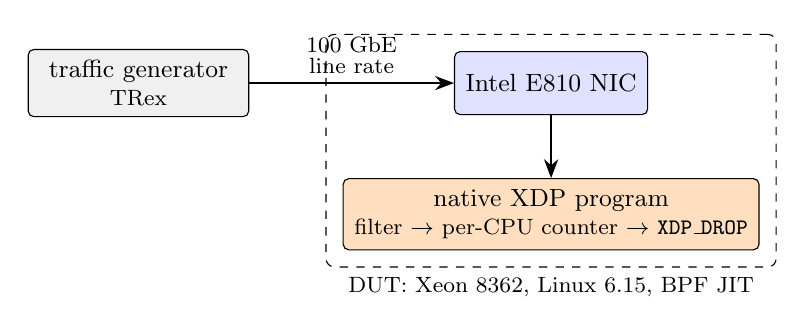
\begin{tikzpicture}[
  font=\small,
  box/.style={draw, rounded corners=2pt, align=center, inner sep=4pt, minimum height=8mm},
  gen/.style={box, fill=gray!12, minimum width=28mm},
  nic/.style={box, fill=blue!12, minimum width=24mm},
  prog/.style={box, fill=orange!25, minimum width=50mm},
  arr/.style={-{Stealth[length=2.4mm]}, semithick},
]

% --- traffic generator ---
\node[gen] (gen) at (0,0) {traffic generator\\[-1pt] {\footnotesize TRex}};

% --- DUT NIC and XDP program ---
\node[nic, right=26mm of gen] (nic) {Intel E810 NIC};
\node[prog, below=8mm of nic] (xdp)
  {native XDP program\\[-1pt]
   {\footnotesize filter $\rightarrow$ per-CPU counter $\rightarrow$ \texttt{XDP\_DROP}}};

% --- DUT enclosure ---
\node[draw, dashed, rounded corners=3pt, inner sep=6pt,
      fit=(nic)(xdp),
      label={[font=\small]below:{\footnotesize DUT: Xeon 8362, Linux 6.15, BPF JIT}}] (dut) {};

% --- link and internal path ---
\draw[arr] (gen.east) -- node[above, font=\footnotesize, align=center]
  {100 GbE\\[-2pt] line rate} (nic.west);
\draw[arr] (nic.south) -- (xdp.north);

\end{tikzpicture}
\end{document}
